\section{Introduction}

\begin{itemize}
    \item \textbf{Artificial Intelligence:} the science to make things smart
    \item \textbf{Machine Learning:} building machines that can learn
    \item \textbf{Deep Learning:} class of ML algorithms
\end{itemize}
\begin{figure}[h]
    \centering
    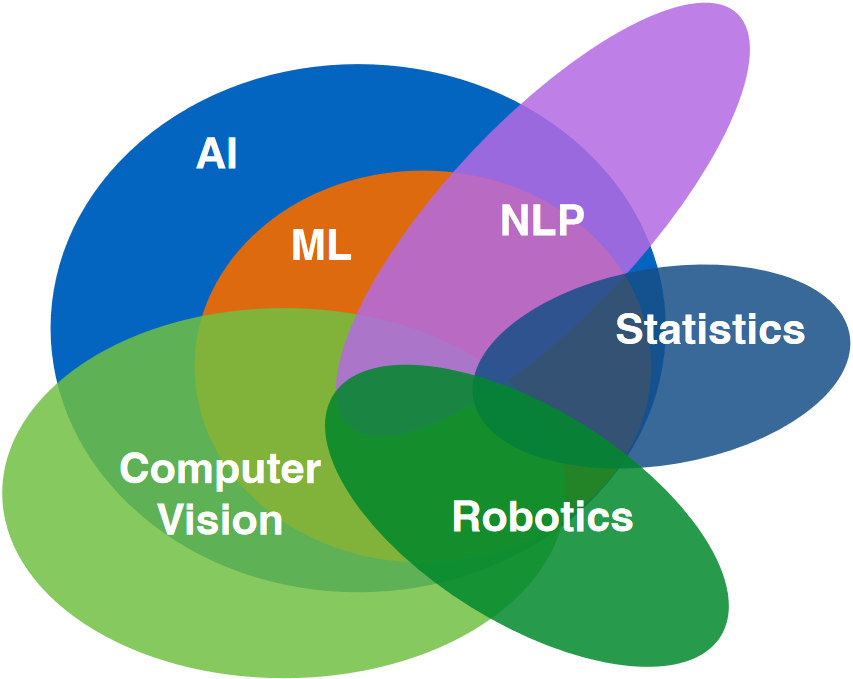
\includegraphics[width=0.4\textwidth]{images/AI.png}
    \caption{Artificial Intelligence}
\end{figure}

\subsection{Artificial Intelligence}
\begin{mdframed}
    J.McCarthy 1956 definition: the science and engineering of making intelligent machines.
\end{mdframed}
\begin{mdframed}
    Modern definition: the ability of a digital computer or computer-controlled robot to perform tasks commonly associated with intelligent beings.
\end{mdframed}

\subsection{Machine Learning}
\begin{mdframed}
    Arthur Lee Samuel 1959 definition: ML is the fields of study that gives computers the ability to learn without being explicitly programmed.
\end{mdframed}
\begin{mdframed}
    Tom Mitchell 1998 definition: A computer program is said to learn from experience $E$ with respect to some class of tasks $T$ ans performance measure $P$, if its performance at tasks in T, as measured by $P$, improves with experience $E$.
\end{mdframed}

\subsection{Learning Algorithm}
The learning algorithm is an algorithm that is able to learn from data. There are 3 main ingredients:
\begin{itemize}
    \item \textbf{Task}
    \begin{itemize}
        \item Is described in terms of how the machine learning algorithm should process an example
        \item How is an example represented? as a collection of features
    \end{itemize}
    \item \textbf{Performance Measure}
    \begin{itemize}
        \item How good is the machine learning system? we need to measure its performance
        \item The performance measures depends on the task
    \end{itemize}
    \item \textbf{Experience}
    \begin{itemize}
        \item The experience is provided by the available data
    \end{itemize}
\end{itemize}

\subsection{Bias}
\begin{mdframed}
    \textbf{Inductive Bias:} all the assumptions about the nature of the target function and its selection.
\end{mdframed}
Example of Inductive Bias:
\begin{itemize}
    \item \textbf{Linear regression:} assume that the output or dependent variable is related to independent variable linearly
    \item \textbf{Nearest neighbors:} assume that most of the cases in a small neighborhood in feature space belong to the same class
\end{itemize}
\begin{mdframed}
    \textbf{Algorithmic Bias:} It describes systematic and repeatable errors in a system that create unfair outcomes, such as privileging one arbitrary group of users over others.
\end{mdframed}
\subsubsection{Bias vs Variance}
\begin{multicols}{2}
    \begin{flushleft}
        The bias error is produced by weak assumptions in the learning algorithm. 
    \end{flushleft}
    \begin{mdframed}
        \textbf{Underfitting:} high bias can cause an algorithm to miss the relevant relations between features and target outputs.
    \end{mdframed}
    \columnbreak
    The variance is an error produced by an over-sensitivity to small fluctuations in the training set.
    \begin{mdframed}
        \textbf{Overfitting:} high variance can cause an algorithm to model the random noise in the training data, rather than the intended outputs.
    \end{mdframed}
\end{multicols}
\begin{figure}[h]
    \centering
    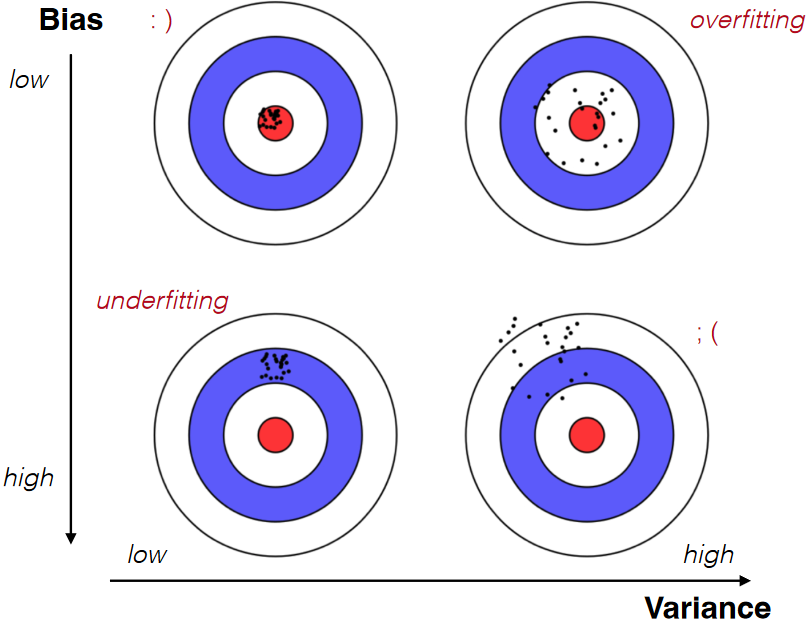
\includegraphics[width=0.7\textwidth]{images/Bias.png}
    \caption{Bias vs Variance}
\end{figure}

\newpage